\documentclass[11pt,letterpaper]{article}
\usepackage[lmargin=1in,rmargin=1in,tmargin=1in,bmargin=1in]{geometry}
\usepackage{../style/homework}
\usepackage{../style/commands}
\setbool{quotetype}{false} % True: Side; False: Under
\setbool{hideans}{false} % Student: True; Instructor: False

\newcommand{\blank}[1]{\underline{\hspace{#1}}} % Blank Underline
\newcommand{\ansun}[2]{\underline{\hspace{#1}#2\hspace{#1}}} % Answer Underline

% -------------------
% Content
% -------------------
\begin{document}

\homework{9: Due 10/12}{We will always have STEM with us. Some things will drop out of the public eye and will go away, but there will always be science, engineering, and technology. And there will always, always be mathematics.}{Katherine Johnson}

% Problem 1
\problem{10} For each of the following functions, determine whether the function is injective, surjective, or bijective. Be sure to fully justify your answer.
	\begin{enumerate}[(a)]
	\item $f: \mathbb{R} \to \mathbb{R}$, $f(x)= 7 - 3x$
	\item $g: \mathbb{R} \to \mathbb{R}^{\geq 0}$, $g(x)= x^2 + 1$
	\item $h: \mathbb{R}^2 \to \mathbb{R}^2$, $h(x, y)= (x - 2y, -2x + 4y)$
	\item $k: [0, \infty) \to \mathbb{R}$, $k(x)= 6 - x^2$
	\end{enumerate} \pspace

\sol 
\begin{enumerate}[(a)]
\item The function $f$ is linear. We know that any non-constant linear function $\ell: \mathbb{R} \to \mathbb{R}$ is bijective. Because $f$ is not constant (because $m= -3 \neq 0$), we know that $f$ is bijective. By definition, bijective functions are injective and surjective, so that $f$ is both injective and surjective. We can also prove this directly. To show that $f$ is injective, we need to show that if $f(x)= f(y)$, then $x= y$. If $f(x)= f(y)$, then\dots
	\[
	\begin{gathered}
	f(x)= f(y) \\
	7 - 3x= 7- 3y \\
	-3x= -3y \\
	x= y
	\end{gathered}
	\]
Therefore, $f$ is injective. To show that $f$ is surjective, given any $y \in \mathbb{R}$, we need to find an $x$ such that $f(x)= y$. Fix $y \in \mathbb{R}$, and define $x:= \frac{7 - y}{3}$. But then\dots
	\[
	f(x)= f \left( \dfrac{7 - y}{3} \right)= 7 - 3 \left( \dfrac{7 - y}{3} \right)= 7 - (7 - y)= 7 - 7 + y= y
	\]
Therefore, $f$ is surjective. Because $f$ is injective and surjective, $f$ is bijective. Alternatively, because every horizontal line intersects the graph of $f$ at least once, $f$ is surjective. Because every horizontal line intersects the graph of $f$ at most once, $f$ is injective. Finally, because every horizontal line intersects the graph of $f$ exactly once, $f$ is bijective. \pspace

\item The function $g$ is not surjective or injective. To see that $g$ is not surjective, fix $0 \in \mathbb{R}^{\geq 0}$. If $g(x)= 0$ for some $x$, then $x^2 + 1= 0$. This implies that $x^2= -1$. But $x^2 \geq 0$ for all $x \in \mathbb{R}$. Therefore, there is no $x$ such that $g(x)= 0$. This shows that $g$ is not surjective. To see that $g$ is not injective, observe that $-1, 1 \in \mathbb{R}$ and $-1 \neq 1$, but $g(-1)= 2= g(1)$. Therefore, $g$ is not injective. Because $h$ is not both surjective and injective, $h$ is not bijective. Alternatively, because every horizontal line $y= c$, where $c \in \mathbb{R}^{\geq 0}$, intersects the graph of $g$ at least once, we know that $g$ is surjective. Because the horizontal line at $y= 2$ intersects the graph of $g$ more than once, we know that $g$ is not injective. Because $g$ is not both surjective and injective, $g$ is not bijective. \pspace

\item The function $h$ is not surjective or injective. To see that $h$ is not surjective, consider $(0, 1) \in \mathbb{R}^2$. If there were $(x, y) \in \mathbb{R}^2$ such that $h(x, y)= (0, 0)$, then $(x - 2y, -2x + 4y)= (0, 1)$. But then $x - 2y= 0$ and $-2x + 4y= 1$. The first equality implies that $x= 2y$. Using this in $-2x + 4y= 1$, we have\dots
	\[
	\begin{gathered}
	-2x + 4y= 1 \\
	-2(2y) + 4y= 1 \\
	-4y + 4y= 1 \\
	0= 1
	\end{gathered}
	\]
which is impossible. Therefore, there is no $(x, y) \in \mathbb{R}^2$ such that $h(x, y)= (0, 1)$, which shows that $h$ is not surjective. So see that $h$ is not injective, observe that $(0, 0), (2, 1) \in \mathbb{R}^2$ and $(0, 0) \neq (2, 1)$, but $h(0, 0)= (0, 0)= h(2, 1)$. Therefore, $h$ is not injective. Because $h$ is not both surjective and injective, $h$ is not bijective. \pspace

\item The function $k$ is not surjective or injective. To see that $k$ is not surjective, fix $7 \in \mathbb{R}$. If there $x \in [0, \infty)$ such that $k(x)= 7$, then\dots
	\[
	\begin{gathered}
	k(x)= 7 \\
	6 - x^2= 7 \\
	-x^2= 1 \\
	x^2= -1
	\end{gathered}
	\]
Because $x^2 \geq 0$ for all $x \in \mathbb{R}$, it is impossible that $x^2= -1$. Therefore, there is no $x \in \mathbb{R}$ such that $k(x)= 7$, which shows that $k$ is not surjective. To see that $k$ is injective, suppose that $k(x)= k(y)$. Then\dots
	\[
	\begin{gathered}
	k(x)= k(y) \\
	6 - x^2= 6 - y^2 \\
	-x^2= -y^2 \\
	x^2= y^2 \\
	x= \pm y
	\end{gathered}
	\]
Because $x= \pm y$, either $x= y$ or $x= -y$. Because $x, y$ are not both zero, if $x= -y$, then $x, y$ have opposite signs. But because $x, y \in [0, \infty)$, that is not possible. Therefore, it must be that $x= y$, so that $k$ is injective. Because $k$ is not both surjective and injective, $k$ is not bijective. Alternatively, because not every horizontal line intersects the graph of $k$ at least once, $k$ is not surjective. Because every horizontal line intersects the graph of $k$ at most once, $k$ is injective. Because $k$ is not both surjective and injective, $k$ is not bijective.  
\end{enumerate}



\newpage



% Problem 2
\problem{10} Let $A= B= \mathbb{R}$. Consider the function $f: A \to B$ given by $f(x)= x^2 - 4x + 7$.
	\begin{enumerate}[(a)]
	\item Sketch a graph of $f(x)$. Be sure your graph includes an interval around the vertex of $f(x)$.
	\item Is $f(x)$ injective? Explain. [Hint: $f(x)= (x - 2)^2 + 3$.]
	\item Is $f(x)$ surjective? Explain. [Hint: $f(x)= (x - 2)^2 + 3$.]
	\item Do your responses in (b) and (c) change if $A= [2, \infty)$? Explain. 
	\item Do your responses in (b) and (c) change if $B= [3, \infty)$? Explain. 
	\end{enumerate} \pspace

\sol
\begin{enumerate}[(a)]
\item Because $f(x)= x^2 - 4x + 7$ is a quadratic function of the form $ax^2 + bx + c$ with $a= 1$, $b= -4$, and $c= 7$. Because $a= 1 > 0$, the parabola opens upwards. The vertex form of $f(x)$ is $(x - 2)^2 + 3$, so that the vertex is $(2, 3)$. This gives the plot below. 
	\[
	\fbox{
	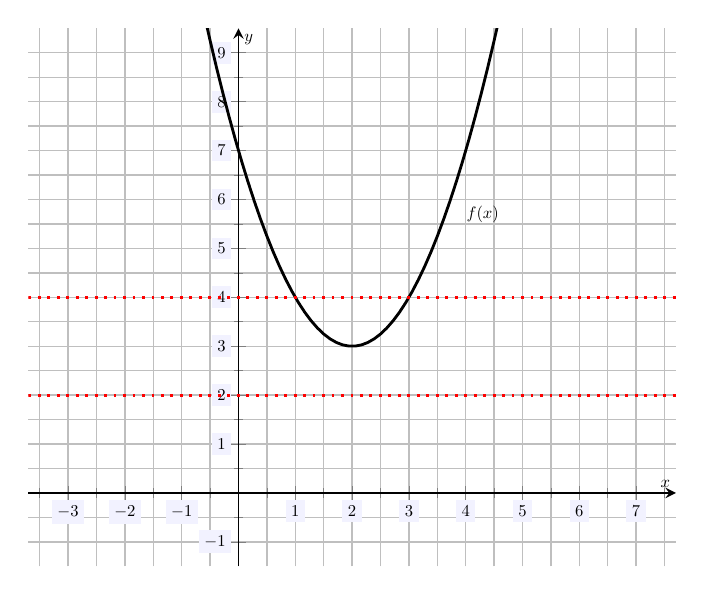
\begin{tikzpicture}[scale=1.2,every node/.style={scale=0.5}]
	\begin{axis}[
	grid=both,
	axis lines=middle,
	ticklabel style={fill=blue!5!white},
	xmin= -3.7, xmax=7.7,
	ymin= -1.5, ymax=9.5,
	xtick={-4,-3,...,8},
	ytick={-1,0,...,9},
	minor x tick num= 1,
	minor y tick num=1,
	xlabel=\(x\),ylabel=\(y\),
	]
	\addplot[domain=-3.5:7.5, samples=100,line width=0.03cm] (x, x^2 - 4*x + 7);
	\node at (4.3,5.7) {$f(x)$};
	
	\draw[line width=0.03cm, red, dotted] (-3.7,4) -- (7.7,4);
	\draw[line width=0.03cm, red, dotted] (-3.7,2) -- (7.7,2);
	\end{axis}
	\end{tikzpicture}
	}
	\]	
	
\item The function $f$ is not injective. We can see that the horizontal line at $y= 4$ intersects the graph of $f$ most than once. Therefore, $f$ is not injective. Alternatively, observe that $1, 3 \in \mathbb{R}$ and $1 \neq 3$, but $f(1)= 4= f(3)$. Therefore, $f$ is not injective. \pspace

\item The function $f$ is not surjective. We can see that the horizontal line at $y= 2$ does not intersect the graph at least once. Therefore, $f$ is not surjective. Alternatively, observe that if $f(x)= 2$, then\dots
	\[
	\begin{gathered}
	f(x)= 2 \\
	(x - 2)^2 + 3= 2 \\
	(x - 2)^2= -1
	\end{gathered}
	\]
Because $(x - 2)^2 \geq 0$ for all $x \in \mathbb{R}$, it is not possible that $(x - 2)^2= -1$. Therefore, there is no $x$ such that $f(x)= 2$, so that $f$ is not surjective. \pspace

\item Observe that if we restrict $f$ to $[2, \infty)$, the graph of $f$ is\dots
	\[
	\fbox{
	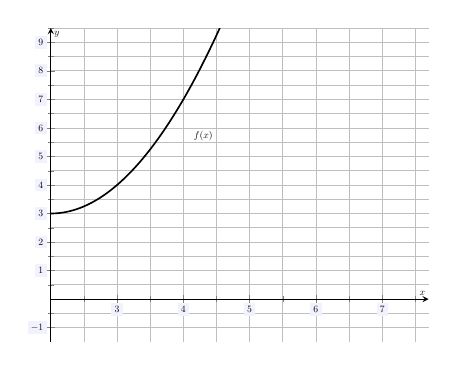
\begin{tikzpicture}[scale=0.7,every node/.style={scale=0.5}]
	\begin{axis}[
	grid=both,
	axis lines=middle,
	ticklabel style={fill=blue!5!white},
	xmin= 2, xmax=7.7,
	ymin= -1.5, ymax=9.5,
	xtick={-4,-3,...,8},
	ytick={-1,0,...,10},
	minor x tick num= 1,
	minor y tick num=1,
	xlabel=\(x\),ylabel=\(y\),
	]
	\addplot[domain=2:7.5, samples=100,line width=0.03cm] (x, x^2 - 4*x + 7);
	\node at (4.3,5.7) {$f(x)$};
	\end{axis}
	\end{tikzpicture}
	}
	\]
Because the horizontal line at $y= 2$ does not intersect the graph of $f$ at least once, $f$ is not surjective. The proofs work the same as in (c). However, because every horizontal line intersects the graph of $f$ at most once, $f$ is injective. To see this algebraically, assume $f(x)= f(y)$. Then\dots
	\[
	\begin{gathered}
	f(x)= f(y) \\
	(x - 2)^2 + 3= (y - 2)^2 + 3 \\
	(x - 2)^2= (y - 2)^2 \\
	x - 2= \pm (y - 2)
	\end{gathered}
	\]
Because $x, y \in [2, \infty)$, $x - 2, y - 2 \geq 0$. But then we cannot have $x - 2= -(y - 2)$ unless $x= y= 2$. Therefore, it must be that $x - 2= y - 2$, so that $x= y$. Therefore, $f$ is injective. \pspace

\item Observe that if we `restrict' $f: [2, \infty) \to [3, \infty)$, the graph of $f$ is\dots 
	\[
	\fbox{
	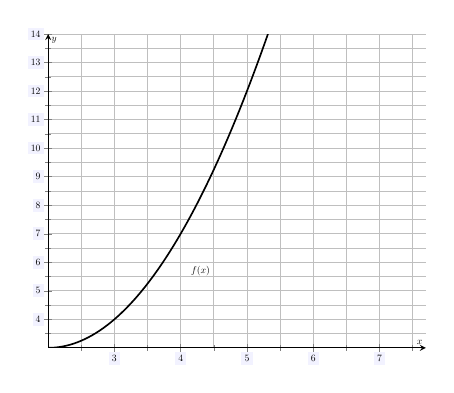
\begin{tikzpicture}[scale=0.7,every node/.style={scale=0.5}]
	\begin{axis}[
	grid=both,
	axis lines=middle,
	ticklabel style={fill=blue!5!white},
	xmin= 2, xmax=7.7,
	ymin= 3, ymax=14,
	xtick={-4,-3,...,8},
	ytick={3,4,...,14},
	minor x tick num= 1,
	minor y tick num=1,
	xlabel=\(x\),ylabel=\(y\),
	]
	\addplot[domain=2:7.5, samples=100,line width=0.03cm] (x, x^2 - 4*x + 7);
	\node at (4.3,5.7) {$f(x)$};
	\end{axis}
	\end{tikzpicture}
	}
	\]
Observe that every horizontal line intersects the graph of $f$ at most once. Therefore, $f$ is injective. Again, the same proofs in (d) apply in this case. Observe that every horizontal line intersects the graph of $f$ at least once. Therefore, $f$ is surjective. Alternatively, choose $y \in [3, \infty)$ and define $x:= 2 + \sqrt{y - 3}$---which is well-defined because $y \geq 3$. Observe\dots
	\[
	f(x)= f \left( 2 + \sqrt{y - 3} \right)= \big( (2 + \sqrt{y - 3}) - 2 \big)^2 + 3= (\sqrt{y - 3})^2 + 3= (y - 3) + 3= y
	\]
Therefore, $f$ is surjective. Because $f$ is both injective and surjective, $f: [2, \infty) \to [3, \infty)$ is a bijection. 
\end{enumerate}



\newpage



% Problem 3
\problem{10} Let $X= \{ 1, 2, 3, 4, 5 \}$, $Y= \{ 1, 2, 3, 4 \}$, and $A= \{ 1, 2, 3 \}$. If $S$ is a set and $\phi: S \to S$ is a function, we say that $s \in S$ is a \textit{fixed point} for $\phi$ if $\phi(s)= s$. Recall that a function $\psi: \mathbb{R} \to \mathbb{R}$ is \textit{strictly increasing} if $\psi(x) < \psi(y)$ for all $x, y \in \mathbb{R}$ with $x < y$.
	\begin{enumerate}[(a)]
	\item Determine a function $F: A \to Y$ that is nondecreasing with no fixed point. Be sure to fully specify the function and justify that $F$ has the required properties. 
	\item Determine a function $G: X \to Y$ such that $G \big|_A= F$ and $G$ is neither surjective nor injective but so that $G$ does have a fixed point. Be sure to fully specify the function and justify that $G$ has the required properties. 
	\item Is $G$ a strictly increasing function? Explain. 
	\end{enumerate} \pspace

\sol 
\begin{enumerate}[(a)]
\item Because $F$ need be a function, each value $F(1)$, $F(2)$, and $F(3)$ need be well-defined, i.e. $F$ need be a function. This implies that there can only be one choice for each of $F(1)$, $F(2)$, and $F(3)$. Because $F \colon A \to Y$ is nondecreasing, we know that $F(1) \leq F(2) \leq F(3)$. Because $F$ cannot have a fixed point, we know that $F(1) \neq 1$. But then $F(1) \geq 2$. Again, because $F$ cannot have a fixed point, we know that $F(2) \neq 2$. But then $F(2) \neq 2$ and $F(2) \geq F(1) \geq 2$. Together, this shows that $F(2) > 2$, i.e. $F(2) \geq 3$ given this codomain. Finally, we know that because $F$ does not have a fixed point, $F(3) \neq 3$. Then $F(3) \neq 3$ and $F(3) \geq F(2) \geq 3$. Together, this shows that $F(3) > 3$, i.e. $F(3) \geq 4$ given this codomain. Therefore, the only possible choices for the function $F$ are given by the relations $\{ (1, 2), (2, 3), (3, 4) \}$, $\{ (1, 3), (2, 3), (3, 4) \}$, and $\{ (1, 4), (2, 4), (3, 4) \}$. Define $F$ via the diagram given below (the first relation given): 
	\[
	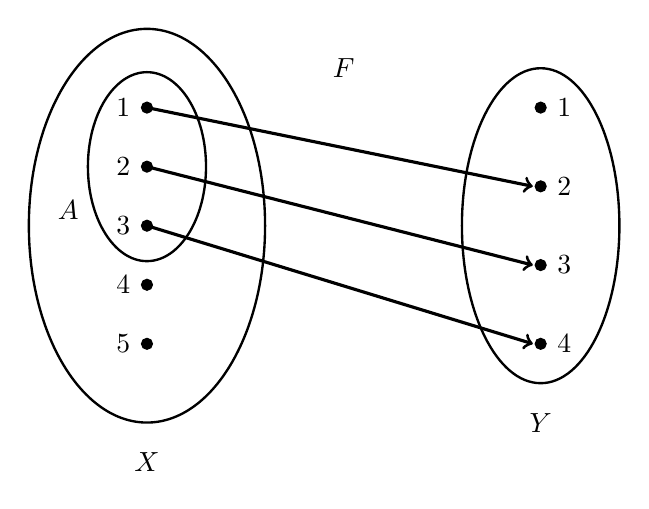
\begin{tikzpicture}
	\node at (2.5,2) {$F$};
	
	% Ellipses
	\draw[line width=0.03cm] (0,0) circle (1.5 and 2.5);
	\draw[line width=0.03cm] (0,0.75) circle (0.75 and 1.2);
	\draw[line width=0.03cm] (5,0) circle (1 and 2);
	
	% Nodes
	\draw[fill=black] (0,1.5) circle (0.07);
	\draw[fill=black] (0,0.75) circle (0.07);
	\draw[fill=black] (0,0) circle (0.07);
	\draw[fill=black] (0,-0.75) circle (0.07);
	\draw[fill=black] (0,-1.5) circle (0.07);
	
	\draw[fill=black] (5,1.5) circle (0.07);
	\draw[fill=black] (5,0.50) circle (0.07);
	\draw[fill=black] (5,-0.5) circle (0.07);
	\draw[fill=black] (5,-1.5) circle (0.07);
	
	% Arrow
	\draw[line width=0.04cm,->] (0,1.5) -- (4.9,0.50);
	\draw[line width=0.04cm,->] (0,0.75) -- (4.9,-0.5);
	\draw[line width=0.04cm,->] (0,0) -- (4.9,-1.5);

	% Labels
	\node at (-0.3,1.5) {$1$};
	\node at (-0.3,0.75) {$2$};
	\node at (-0.3,0) {$3$};
	\node at (-0.3,-0.75) {$4$};
	\node at (-0.3,-1.5) {$5$};
	
	\node at (5.3,1.5) {$1$};
	\node at (5.3,0.5) {$2$};
	\node at (5.3,-0.5) {$3$};
	\node at (5.3,-1.5) {$4$};
	
	\node at (0,-3) {$X$};
	\node at (-1,0.2) {$A$};
	\node at (5,-2.5) {$Y$};
	\end{tikzpicture}
	\]
It is clear that $F$ is a function. Observe that $F(1) \neq 1$, $F(2) \neq 2$, and $F(3) \neq 3$. Therefore, $F$ has no fixed point. Finally, observe that $F(1) \leq F(2) \leq F(3)$ so that $F$ is nondecreasing. \pspace

\item Because $G$ need be a function, each input of $G$ need be well defined. Furthermore, because $G \big|_A= F$, we need choose the same values for $G$ as $F$ on $A$. So we need only extend $F$ to $X$ by defining $F$ at 4 and 5. Now $G$ cannot be surjective so that $G(4) \neq 1$ and $G(5) \neq 1$; otherwise, for every $y \in Y$, there would be $x \in X$ such that $F(x)= y$ and $F$ would be surjective. But $G$ needs a fixed point. Because $5 \in X$ and $5 \notin Y$, $5 \neq G(5) \in Y$ cannot be a fixed point. Therefore, in order for $G$ to have a fixed point, we must choose $G(4)= 4$. But then because $3 \neq 4$ but $G(3)= 4= G(4)$, so that $G$ is not injective. We only need define $G(5)$. We can choose any value in $\{ 2, 3, 4 \}$. We simply choose $G(5)= 4$. The function $G$ is given by $F$ (on the set $A$) and the values at 4 and 5 are given by the lines in red below. 
	\[
	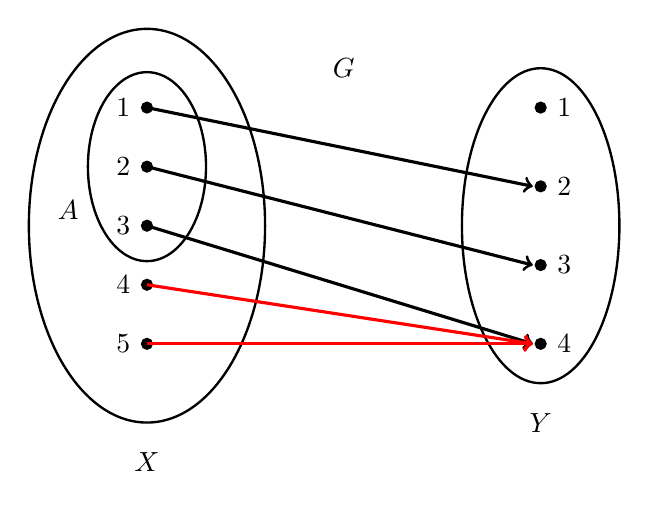
\begin{tikzpicture}
	\node at (2.5,2) {$G$};
	
	% Ellipses
	\draw[line width=0.03cm] (0,0) circle (1.5 and 2.5);
	\draw[line width=0.03cm] (0,0.75) circle (0.75 and 1.2);
	\draw[line width=0.03cm] (5,0) circle (1 and 2);
	
	% Nodes
	\draw[fill=black] (0,1.5) circle (0.07);
	\draw[fill=black] (0,0.75) circle (0.07);
	\draw[fill=black] (0,0) circle (0.07);
	\draw[fill=black] (0,-0.75) circle (0.07);
	\draw[fill=black] (0,-1.5) circle (0.07);
	
	\draw[fill=black] (5,1.5) circle (0.07);
	\draw[fill=black] (5,0.50) circle (0.07);
	\draw[fill=black] (5,-0.5) circle (0.07);
	\draw[fill=black] (5,-1.5) circle (0.07);
	
	% Arrow
	\draw[line width=0.04cm,->] (0,1.5) -- (4.9,0.50);
	\draw[line width=0.04cm,->] (0,0.75) -- (4.9,-0.5);
	\draw[line width=0.04cm,->] (0,0) -- (4.9,-1.5);
	\draw[line width=0.04cm,->,red] (0,-0.75) -- (4.9,-1.5);
	\draw[line width=0.04cm,->,red] (0,-1.5) -- (4.9,-1.5);

	% Labels
	\node at (-0.3,1.5) {$1$};
	\node at (-0.3,0.75) {$2$};
	\node at (-0.3,0) {$3$};
	\node at (-0.3,-0.75) {$4$};
	\node at (-0.3,-1.5) {$5$};
	
	\node at (5.3,1.5) {$1$};
	\node at (5.3,0.5) {$2$};
	\node at (5.3,-0.5) {$3$};
	\node at (5.3,-1.5) {$4$};
	
	\node at (0,-3) {$X$};
	\node at (-1,0.2) {$A$};
	\node at (5,-2.5) {$Y$};
	\end{tikzpicture}
	\] \pspace

\item Examining all the possible choices for $F$ in (a), we observe that we must have $F(3)= 4$. But from (b), we know that we must have $G(3)= F(3)= 4$ and $G(4)= 4$. But then $3 < 4$ but $G(3)= 4 \not< G(4)$ so that $G$ is not strictly increasing. 
\end{enumerate}



\newpage



% Problem 4
\problem{10} Below is a partial proof of the fact that if $f: X \to Y$ is a function and $A, B \subseteq Y$, then $f^{-1}(A \cup B)= f^{-1}(A) \cup f^{-1}(B)$. By filling in the missing portions, complete the partial proof below so that it is a correct, logically sound proof with `no gaps.' \pspace

\noindent \textbf{Proposition.} If $f: X \to Y$ is a function and $A, B \subseteq Y$, then $f^{-1}(A \cup B)= f^{-1}(A) \cup f^{-1}(B)$. \pspace

\textit{Proof.} To prove that $f^{-1}(A \cup B)= f^{-1}(A) \cup f^{-1}(B)$, we need to show \ansun{0cm}{$f^{-1}(A \cup B) \subseteq f^{-1}(A) \cup f^{-1}(B)$} \pspace and \ansun{0cm}{$f^{-1}(A) \cup f^{-1}(B) \subseteq f^{-1}(A \cup B)$}. \pvspace{2\baselineskip}


Clearly, if $f^{-1}(A \cup B)= \varnothing$, then $f^{-1}(A \cup B) \subseteq f^{-1}(A) \cup f^{-1}(B)$. Similarly, if $f^{-1}(A) \cup f^{-1}(B)= \varnothing$, then $f^{-1}(A) \cup f^{-1}(B) \subseteq f^{-1}(A \cup B)$. Assume neither $f^{-1}(A \cup B)$ nor $f^{-1}(A) \cup f^{-1}(B)$ are empty. \pvspace{2\baselineskip}


$f^{-1}(A \cup B) \subseteq f^{-1}(A) \cup f^{-1}(B)$: Let $x \in$ \ansun{0.52cm}{$f^{-1}(A \cup B)$}. But then $f(x) \in A \cup B$. This implies \pspace that either $f(x) \in$ \ansun{1.35cm}{$A$} or $f(x) \in$ \ansun{1.35cm}{$B$}. \pspace

	\hspace{1cm} Case 1, $f(x) \in$ \ansun{1.35cm}{$A$}: If $f(x) \in A$, then \ansun{1.38cm}{$x$} $\in f^{-1}(A)$. But then \pspace \hspace{1cm} $x \in$ \ansun{0.55cm}{$f^{-1}(A) \cup f^{-1}(B)$}. \pvspace{1cm}

	\hspace{1cm} Case 2, $f(x) \in B$: If $f(x) \in B$, then $x \in$ \ansun{0.9cm}{$f^{-1}(B)$}. But then $x \in f^{-1}(A) \cup f^{-1}(B)$. \pvspace{1cm}

Therefore, if $x \in f^{-1}(A \cup B)$, we know that $x \in$ \ansun{1.07cm}{$f^{-1}(A) \cup f^{-1}(B)$}. This shows \pspace that $f^{-1}(A \cup B) \subseteq f^{-1}(A) \cup f^{-1}(B)$. \pvspace{2\baselineskip}


$f^{-1}(A) \cup f^{-1}(B) \subseteq f^{-1}(A \cup B)$: Suppose that \ansun{0.72cm}{$x \in f^{-1}(A) \cup f^{-1}(B)$}. This implies \pspace that $x \in f^{-1}(A)$ or $f^{-1}(B)$. \pspace

	\hspace{1cm} Case 1, \ansun{0.55cm}{$x \in f^{-1}(A)$}: If $x \in f^{-1}(A)$, then $f(x) \in A$. But then $f(x) \in$ \ansun{0.97cm}{$A \cup B$}. \pspace \hspace{1cm} This shows that $x \in f^{-1}(A \cup B)$. \pvspace{1cm}

	\hspace{1cm} Case 2, $x \in f^{-1}(B)$: If $x \in f^{-1}(B)$, then $f(x) \in$ \ansun{1.32cm}{$B$}. But then $f(x) \in f(A \cup B)$. \pspace \hspace{1cm} This shows that $x \in$ \ansun{0.50cm}{$f^{-1}(A \cup B)$}. \pvspace{2\baselineskip}

Therefore, if $x \in f^{-1}(A) \cup f^{-1}(B)$, we know that $x \in f^{-1}(A \cup B)$. This shows that \ansun{0cm}{$f^{-1}(A) \cup f^{-1}(B) \subseteq f^{-1}(A \cup B)$}. \pvspace{2\baselineskip}


But then we have shown that \ansun{0cm}{$f^{-1}(A \cup B) \subseteq f^{-1}(A) \cup f^{-1}(B)$} and \ansun{0cm}{$f^{-1}(A) \cup f^{-1}(B) \subseteq f^{-1}(A \cup B)$}. \pspace Therefore, $f^{-1}(A \cup B)= f^{-1}(A) \cup f^{-1}(B)$. 


\end{document}